\documentclass[a4paper]{jpconf}
\usepackage[utf8]{inputenc}
\usepackage{graphicx}
\usepackage{lmodern}
\bibliographystyle{iopart-num}


\begin{document}
\title{The Neutron Monitor Control Panel}

\author{O. García-Población$^{1,2}$, H. Ivanov$^2$, I. García-Tejedor$^{1,2}$,
J. J. Blanco$^{1,2}$, J. Medina$^{1,2}$, R. Gómez-Herrero$^{1,2}$, E.
Catalán$^{1,2}$ and D. Radchenko$^{2}$}

\address{$^1$ Space Research Group, University of Alcalá, Spain}
\address{$^2$ Castilla-La Mancha Neutron Monitor, Parque Tecnológico de Guadalajara, Spain}

\ead{oscar.gpoblacion@uah.es}

\begin{abstract}
    This work presents the current status and future plans of NMCP, a new
    software developed to aid the operator in typical station maintenance and
    configuration operations. This software is integrated with the new NOAS
    data acquisition system and can be accessed using a supported web browser.
    If features a visual inspection tool to help the operator to identify
    spikes in the data, trace the origin of the spike back to the raw readings
    of each counter tube and pressure reading, and mark the data as invalid in
    the Neutron Monitor Database if desired. The software also provides
    information about station operation status, some descriptive statistics
    about current data being recorded and, in the future, will provide an
    interface to configure station parameters.
\end{abstract}

\section{Introduction}

Neutron Monitor data is widely used by researchers in different research fields
not necessarily related to cosmic rays. That's why the NMBD\cite{NMDB2011}
puts effort into delivering data with the best quality possible. The data is
also used in real time GLE alarm systems and other real time applications;
therefore, the data quality protocol must be applied in real time. Eventually,
the data will be revised by a human supervisor to ensure the correct behaviour
of the quality protocol. By quality protocol we refer to all the methods and
techniques used such as:

\begin{itemize}
	\item   Detection of abnormal data, commonly referred to as spikes.
    \item   Detection of inactivity, which will lead to a notification to the
        team responsible for the neutron monitor station.
    \item   Monitor neutrons are usually formed by 18 counter tubes. A
        malfunction in a single tube won't affect the overall value measured by
        the neutron monitor but it's not something desirable. This leads us to
        the need of monitoring and detection of malfunctions separately in each
        of the tubes.  
    \item	Detection of changes with respect to the historical activity.
        Since changes in the immediate environment or the instruments can cause
        overall changes in the measured values of a monitor neutron, detecting
        and correcting those changes is desirable.
    \item 	Comparing the data from one NM station to the data of different
        nearby NM stations. Detecting isolated events in one NM station
        indicates that there is a malfunction in that NM station.	
\end{itemize}

Once the corrupted data is detected, the cause of such data corruption can often 
be traced down to its cause. Most of the times those malfunctions are caused by the instruments
forming the data acquisition system, so detecting the corrupt data and its cause
helps us improve and learn more about it. In order
to ease the detection of the corrupt data we are working in the
development of a Web tool which will help us detect these corruptions. The Web
application makes use of dynamically generated plots which are designed to highlight
possible corrupted data.

This software is currently running for testing in the second release of the data
acquisition system\cite{Garcia2014} designed for the CaLMa\cite{Medina2013} and
KIEL2 stations.


\section{System architecture}

There are two main elements in the architecture: a client that requests and
consumes data using a web browser, and a system that collects and serves the
data, which in this system is the data acquisition system. The figure
\ref{fig:arch} shows a block diagram with all the components involved along with
its relationships. This separation of roles follows the client-server design
pattern\cite{wiki:ClientServer}.

The software architecture is based on the Model-View-Controller (MVC) software
design pattern\cite{wiki:MVC}. This pattern encourages the separation between
the data, the data processing and the data representation. 

The view component is in charge of the data representation and the user
interface. In our system, this component is mainly executed by the client in a
web browser, which is not only a convenient graphical output device but
also provides a way to interact with the user. In response to these
interactions, the browser makes requests to a server which answers back with new
data to be represented.

The model component is located on the server side, in the data acquisition
system. This model comprises all the data captured from each counter tube and
the algorithms used to process these data, such as atmospheric pressure
corrections, sanity controls, editors to combine all the readings into a single
one, etc.

Several controllers adapt and serve the model data as REST-like web services,
using JSON for data representation. This web services are designed to be a
documented API for accessing the station information and services, allowing
third party applications to be further developed. The main consumer of this API
right now is the spike tool, which is used to track and mark anomalous surges in
the data from the station. The next section describes this tool in detail.

\begin{figure}[h]
    \centering
    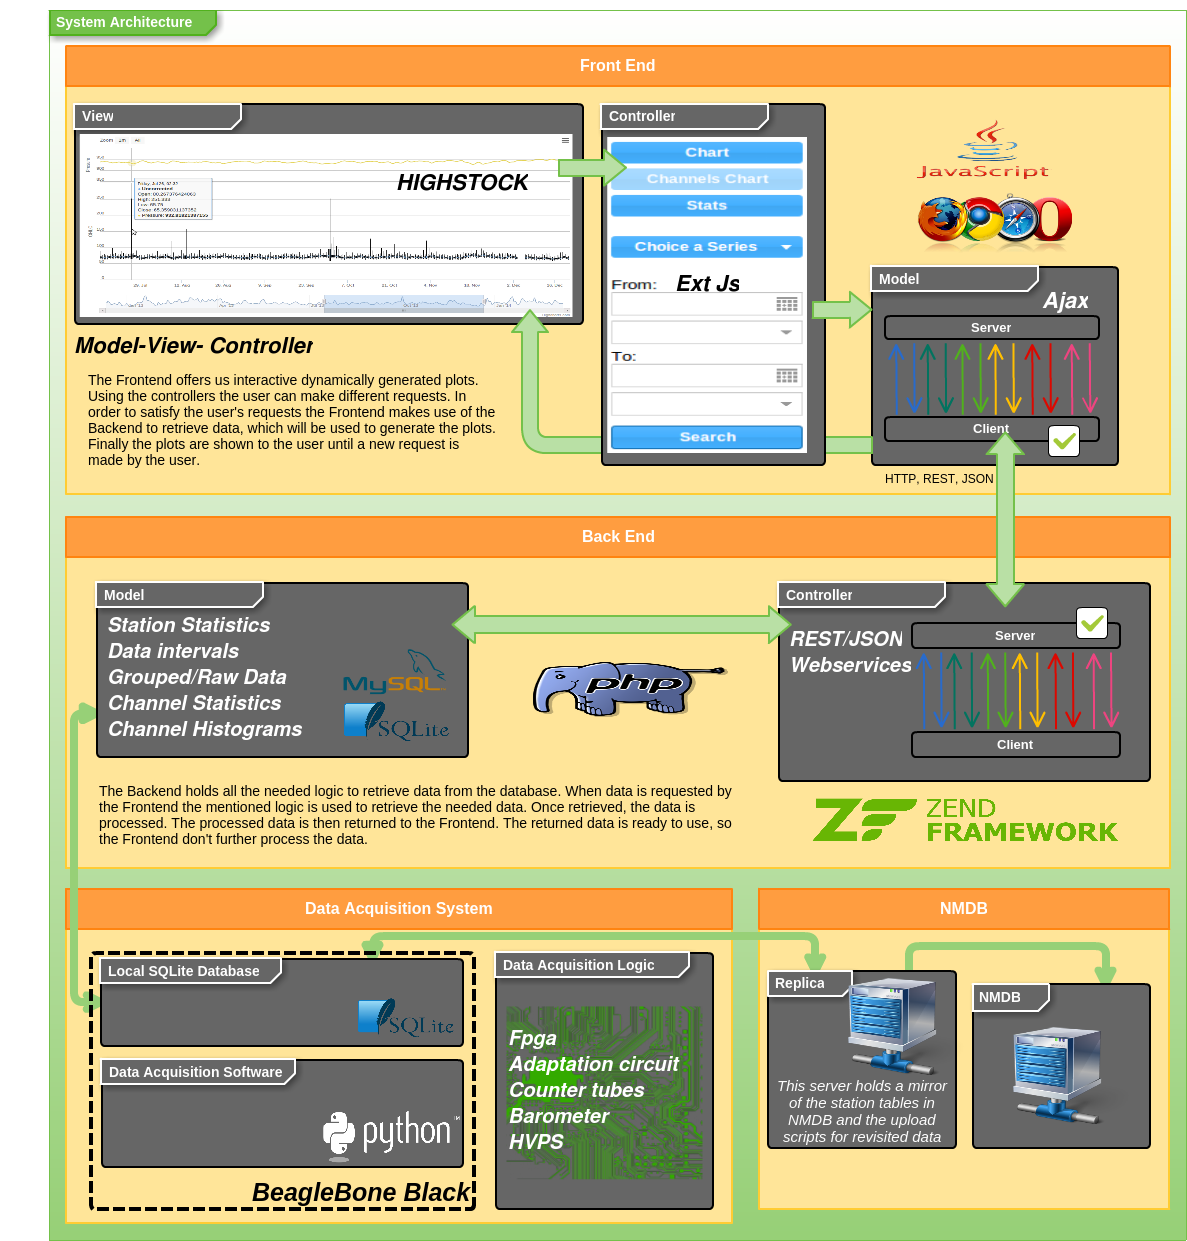
\includegraphics[keepaspectratio, width=1\textwidth]{./resources/Architecture.png}
    \caption{Architecture}
    \label{fig:arch}
\end{figure}

\section{The spike tool}

Currently the Spike Tool consists of three modules, Spike, SpikeCorrected and
ChannelStats. Spike and SpikeCorrected are very similar, but SpikeCorrected works
with a different set of data and has some extra functionality.

The Spike module offers a highly interactive chart in which the spikes are easy
to trace. Initially the chart displays a large set of data, and some kind of
data grouping is needed. Just averaging the data flattens the spikes.
The Candlestick chart is used to prevent the aforementioned problem, as this way the
max and min values can be easily distinguished. Eventually when a short interval
of data is requested and no grouping is needed to display it, the chart
will automatically switch to a line chart.

As mentioned above the chart is highly interactive, and offers a very intuitive
zooming functionality. Clicking and dragging through an interval of the chart will
raise a zoom event, and depending on the drag direction the event will be zoomed In
or Out. The chart also offers a navigator which allows us to navigate forwards or
backwards in time. Datetime input fields are available too, which allows the user to
plot a specific time interval.

At first the uncorrected data is used to generate the charts, but we are given
the chance to choose between Uncorrected data and Efficiency and Pressure corrected
data. The atmospheric pressure is also plotted, which helps us to evaluate how the
atmospheric pressure affects the measurements of our Neutron Monitor station.

Once we have a spike located, we can see the raw reading of the counter tubes,
which allows us to better track the spike. Due to the fact that there is 18
channels this option is available only when no data grouping is needed.

As said before, the SpikeCorrected module is very similar to the Spike module
which was explained above. First of all, this module makes use of a diferent
set of data. The Spike module uses the raw data which comes from the data
adquisition system while SpikeCorr uses the revisited data, and also provides
the ability to update that revisited data.

Clicking on a value in the chart will mark the clicked data, which is
stored in a grid. The data in the grid can be later submitted to the revisited
set of data, which means that the mentioned data will be considered invalid and
treated as void in the future.

The grid which contains the marked data can be seen on a separate window, which
can be show and hidden when needed. The window also contains all the
controls needed for submitting and unmarking the marked data.

The last module, ChannelStats, is intended to give informatión about the
different channels separately, so that we can identify malfunctions on isolated
channels. The module offers various statistics for user defined time intervals,
among which the simplest are the average value, minimum/maximum
values and standard deviation.

The ChannelStats module offers distribution charts, too. Histograms with the
channels' raw data are ploted in the requested time intervals. The chart is
highly interactive, and the series can be shown, hidden and highlighted. Currently
we are working on this module.

\begin{figure}[h]
    \centering
    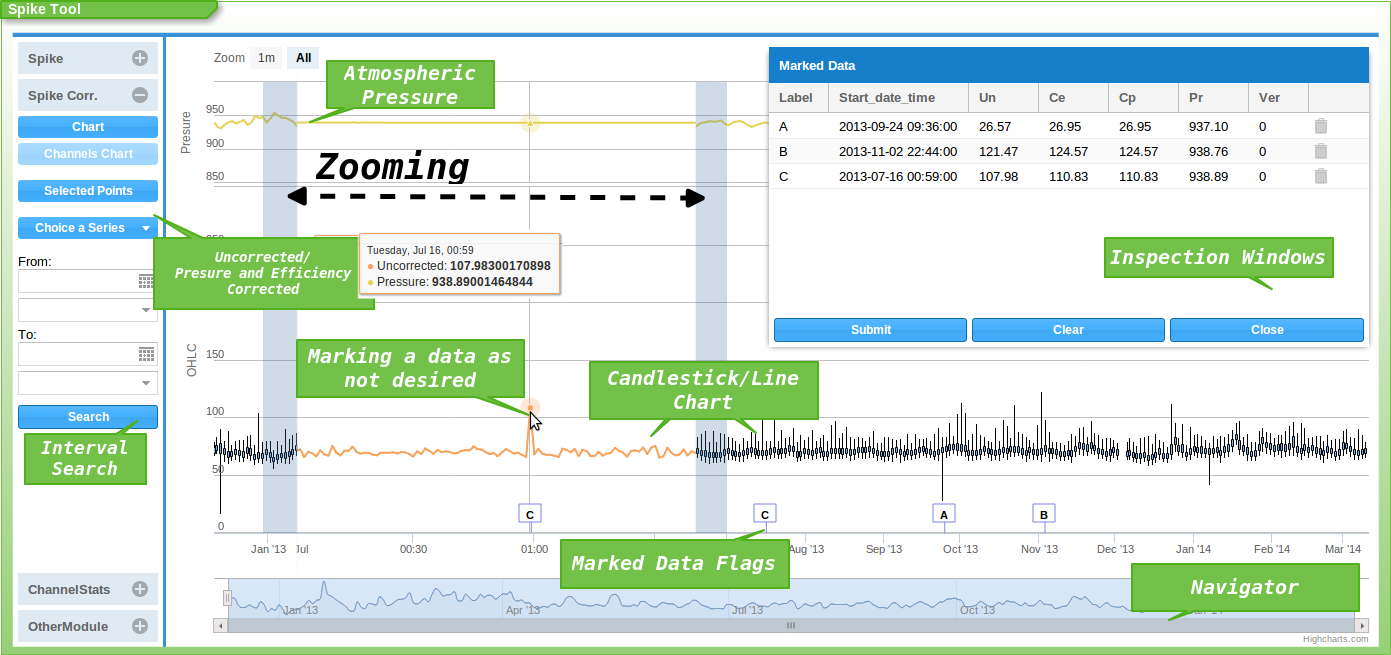
\includegraphics[keepaspectratio, width=1\textwidth]{./resources/SpikeTool.png}
    \caption{Spike Tool}
    \label{fig:arch}
\end{figure}

\section{Future work}

The neutron monitor control panel is a natural evolution of the new data
acquisition system designed for neutron monitors and is under active
development to add new useful features in the near future. Some of these future
features are summarized below.

\begin{description}
    \item[Online statistics] The control panel will include a module for
        descriptive statistics that will be calculated in real time from the
        counter tubes raw readings. This will help to identify drifts in the
        behavior of the detectors and to apply the appropriate actions to
        maintain data quality.
    \item[Station reconfiguration] This will allow the operator to disconnect a
        counter from the station without affecting global station count. This
        can be useful to perform maintenance operations such as counter tube
        diagnostics. 
    \item[Station parameter setup] New electronics allow the remote control of
        some parameters, for example the high voltage power supply set point,
        the remote database for data upload, backup policies, etc.
    \item[Alarms and push notifications] When connectivity allows it, it will
        be possible to configure alarms and notifications to recipients using
        the new push mobile technologies. For example, if the station is no
        longer uploading data to NMDB or if data is out of quality standards
    \item[Detector response histogram] A new design from the New
        Hampshire University of the front-end amplifiers provides a pulse whose
        width is proportional to the energy of the incident particle. The new
        FPGA IP-core running in the NOAS, the second version of our data
        acquisition system, is able to read these pulses and to generate an
        histogram with the distribution of the pulses energy over a given time
        interval. This will enable a mechanism for non-intrusive diagnostics of
        the counter tubes. 
\end{description}


\subsection*{Acknowledgments} 

The authors would like to thank the OMNIweb team and the Neutron Data Base for
the use of their data. This work has been partially supported by Ministerio de
Ciencia y Tecnologia through the project AYA2012-39810-C02-01 Authors want also
to acknowledge to the Observatoire Midi- Pyrenees for putting the BP28 tubes at
our disposition,enabling us to start our station and The authors would like to
thank Karl-Ludwig Klein from the L’Observatoire de Paris and Francis Beigbeder
from the Observatoire Midi-Pyrenees for putting the BP28 counters at our
disposition, enabling us to start our station. Also thank to Christian T.
Steigies, Bernd Heber, Eckart Böhm and Cesar Martín from the Christian
Albrechts University in Kiel,Germany, for their help in our research and new
improvements.


\section*{References}
\bibliography{iopart-num} 

\end{document}


